%% josis.tex 1.4   2016-09-15    JoSIS latex template
%------------------------------------------------------------------
% Filename: josis_template.tex
%
% This file is intended as a template for typesetting articles for the
%
%                        Journal of Spatial Information Science.
%
% Please edit this template to generate your own formatted manuscripts
% for submission to JOSIS. See http://josis.org for further details.
%


%%% JOSIS checks in typesetting
%%% * All titles and sections lower case *EXCEPT short title  [ ]
%%% * Remove author postal addresses, only have geographic places and institutions [ ] 
%%% * Consistent use of Section, Figure, Table (capitalized and in full) [ ]
%%% * 10 keywords (and all lower case) [ ]
%%% * Remove all avoidable footnotes [ ]
%%% * Use double quotation marks (``'' not "" or `') [ ]
%%% * Punctuation inside quotations [ ]
%%% * E.g. and i.e. followed by comma [ ]
%%% * cf. followed by tilde [ ]
%%% * Itemize and enumerate correctly punctuated [e.g., "1. x, 2. y, and 3. x." ]
%%% * And/or lists using American English punctuation (e.g., "x, y, and z") [ ] 
%%% * Bibliography (e.g., en-dashes for number ranges, consistent "Proc.~" for Proceedings of..., etc.) []
%%% * Acknowledgment style use section* [ ] 
%%% * et al. no italics, but with dot  [ ] 
%%% * All captions end with full stop  [ ] 
%%% * Table captions under, not over table  [ ]
%%% * Adjust urls with burlalt [ ] 
%%% * Check correct use of hyphens, emdashes, endashes  [ ]
%%% * Perform spell check  [ ] 

%%% JOSIS checks directly before publication 
%%% Check DOI, page numbers on article and web site. [ ]
%%% Update web site with final title, abstract, keywords. [ ] 
%%% Build with distiller for DOI links. [ ]


% Required documentclass definition for JOSIS
\documentclass{josis}
\usepackage{hyperref}
\usepackage[hyphenbreaks]{breakurl}
\usepackage{booktabs}
\usepackage{stmaryrd}
\usepackage[T1]{fontenc}
\usepackage{cite}
\usepackage{subcaption}

% Suggested packages for algorithm formatting
\usepackage{algorithm}
%\usepackage{algorithmic}
\usepackage{algpseudocode}
\usepackage{pythonhighlight}

\usepackage{amssymb,amsmath}
%\usepackage[table]{xcolor}
\usepackage{lastpage}
\renewcommand{\topfraction}{0.9} 
\renewcommand{\textfraction}{0.1}
% Page setup and overhangs
\sloppy
\widowpenalty=10000
\clubpenalty=10000
\hyphenpenalty=75

% Article details for accepted manuscripts will be added by editorial staff
% Omit year if article in press
% Omit number if article under review
\josisdetails{%
   number=2, year=2025, firstpage=1, lastpage=\pageref{LastPage}, 
  doi={IUIT-2025},
  % received={December 24, 2015}, 
   %returned={February 25, 2016},
   %revised={July 13, 2016},
   %accepted={September 5, 2016},
   }

%\newcommand{\mydoi}[1]{\href{http://dx.doi.org/#1}{doi:\protect\detokenize{#1}}}

%\renewcommand{\UrlLeft}{http:\sslash}
%\DeclareUrlCommand\myurl{\def\UrlLeft{}\def\UrlRight{}%
%\urlstyle{tt}}

\urlstyle{rm}
\makeatletter
% Inspired by http://anti.teamidiot.de/nei/2009/09/latex_url_slash_spacingkerning/
% but slightly less kern and shorter underscore
\let\UrlSpecialsOld\UrlSpecials
\def\UrlSpecials{\UrlSpecialsOld\do\/{\Url@slash}\do\_{\Url@underscore}}%
\def\Url@slash{\@ifnextchar/{\kern-.11em\mathchar47\kern-.2em}%
    {\kern-.0em\mathchar47\kern-.08em\penalty\UrlBigBreakPenalty}}
\def\Url@underscore{\nfss@text{\leavevmode \kern.06em\vbox{\hrule\@width.3em}}}
\makeatother

\hypersetup{
colorlinks=true,
linkcolor=black,
citecolor=black,
urlcolor=black
} 

% Add the running author and running title information
\runningauthor{\begin{minipage}{.9\textwidth}\centering Adithya Ajith, Namitha K, Elin Grace John \end{minipage}}
\runningtitle{AI-Powered Interactive Learning Assistant for Classrooms}

% Document begins
\begin{document}
%\setcounter{page}{33}


% Insert your own title
\title{AI-Powered Interactive Learning Assistant for Classrooms}

% Insert your manuscipts authors, affiliations, and addresses
\author{Adithya Ajith}
\author{Namitha K }
\author{Elin Grace John}\affil{Saintgits Group of Institutions, Kottayam, Kerala}
\date{}
\maketitle
% Add 5-10 keywords for every submission
\keywords{ Multimodal AI, NLP, OCR, Voice-Based Queries, Text Input, OpenVINO, Streamlit, Educational Technology, AI in Classrooms, Real-Time Inference


}
% Add a short abstract of 150-250 words 
\begin{abstract}
This project, titled Mentora, presents an AI-based educational assistant designed to enhance student learning through multi-modal interaction. The system allows users to ask academic questions via text input, image uploads, or voice commands and provides intelligent responses using a locally optimized language model. The backend is powered by a quantized neural-chat model executed through OpenVINO for efficient CPU performance, while Tesseract OCR handles text extraction from images. Mentora supports both online and offline modes text and image queries can be processed entirely offline, ensuring accessibility in low-connectivity environments. Voice input, however, relies on browser-based speech recognition and functions only with an internet connection. The web-based interface is intuitive and student-friendly, guiding users through a step-by-step experience from identity input to question-answering. By combining AI, computer vision, and speech technologies, Mentora offers a robust, accessible, and engaging platform to assist students in their everyday learning journey.

\end{abstract}
% Your main text begins here. 
\section{Introduction}
Mentora is a smart, AI-powered educational assistant designed to support students in learning by providing instant answers to their questions through text, image, or voice input. Built with a user-friendly web interface and powered by the neural-chat language model optimized using OpenVINO, Mentora can function efficiently both online and offline for text and image-based queries. Users can type their questions or upload handwritten or printed material as images, which are processed locally using Tesseract OCR and passed to the language model for accurate responses without needing an internet connection. However, voice input relies on browser-based speech recognition, which requires an active internet connection to function. This hybrid setup makes Mentora a versatile tool for learning, especially in environments with limited or inconsistent connectivity, while still offering the convenience of voice interaction when online.
\section{Libraries Used}
In the project for various tasks, following packages are used.
\begin{python}
flask
flask cors
werkzeug.utils 
transformers 
optimum.intel.openvino  
Pillow
pytesseract 
os 
\end{python}
\section{Methodology}
Your project uses multiple integrated methodologies from AI, image processing, and web technologies to deliver a seamless educational assistant experience:\\
\textbf{ Frontend Development:}The frontend is built using HTML, CSS, and JavaScript to create a clean,interactive, and responsive web interface.\\
\textbf{Text Input Handling}:Users can type questions into a textarea, which are sent to the backend via a POST request for processing.\\
\textbf{Image Input Handling}:Users can upload images containing text, which are transmitted to the backend using a FormData POST request.\\
\textbf{Voice Input Handling}:Voice input is implemented using the browser Web Speech API, which requires an active internet connection to convert speech to text.\\
\textbf{Backend Framework}:The backend is developed using Flask, handling API requests for text, image, and voice inputs.\\
\textbf{Model Deployment}:A quantized neural-chat language model is loaded and compiled with OpenVINO for optimized and efficient CPU inference.\\
\textbf{Text Query Processing}:Text questions from the frontend are tokenized, processed through the AI model, and the generated response is returned to the frontend.\\
\textbf{Image Query Processing}:Uploaded images undergo OCR using Tesseract to extract text, which is then sent to the AI model for generating a suitable answer.\\
\textbf{Offline Support}:Both text and image queries are handled locally on the system, allowing them to function without an internet connection.\\
\textbf{Voice Mode Dependency}:Voice input relies on the Web Speech API online service, making it functional only when an active internet connection is available.\\
\textbf{Response Delivery}:AI-generated answers are sent back to the frontend, which dynamically displays the response in the user interface.\\

 
\begin{description}



\end{description} 
\section{Implementation}
The implementation of the Mentora project is based on a modular architecture comprising a Flask-based backend, a web-based frontend, and an OpenVINO-optimized AI language model. The core functionality allows users to interact with the system through three input modes text, image, and voice. The backend runs entirely on local hardware, allowing text and image-based question processing to work even in offline mode. The language model, a quantized version of "neural-chat", is compiled using OpenVINOs inference engine to optimize performance and reduce computational load on the CPU.



The Flask backend is responsible for handling client requests through three primary routes: the root route serves the frontend interface; the /chat endpoint processes text-based questions; and the /upload-image endpoint handles image uploads. For textual input, the question is tokenized using Hugging Face  AutoTokenizer, then passed to the OVModelForCausalLM for inference. When a user uploads an image, the backend uses Tesseract OCR to extract any visible text, which is then treated as a question and forwarded to the same model for a response. All responses are returned to the client in JSON format for rendering on the frontend.





The frontend is designed using HTML, CSS, and vanilla JavaScript to ensure simplicity and responsiveness. It consists of three stages: a splash screen, a user detail form, and the interactive question interface. Once the student submits their name and class, they are taken to the main screen where they can type a question, speak into a microphone, or upload an image. JavaScript handles all client-side logic, including voice recognition using the Web Speech API, API calls using fetch(), and UI updates for displaying AI-generated answers. Text and image-based queries work seamlessly regardless of internet connectivity because the model and OCR engine are hosted locally.



Voice input is handled entirely by the browser and requires an active internet connection. This is due to the Web Speech API relying on cloud-based speech-to-text services for converting voice into text. Once converted, the recognized speech is inserted into the text input field and processed like any other question. Although this feature is limited to online mode, it provides added convenience and accessibility for younger users or those with difficulty typing.



In conclusion, the implementation of Mentora offers a robust, offline-capable learning assistant by integrating computer vision, natural language processing, and voice interaction in a unified system. The use of OpenVINO and Tesseract ensures efficient on-device performance, while the web interface keeps the platform easy to use and accessible to students. Its architecture supports both online and offline modes effectively, making it suitable for use in classrooms with limited connectivity or in rural learning environments.

 
\section{Results \& Discussion}
The AI-powered interactive learning assistant application named Mentora was successfully developed and tested. The system integrates a user-friendly web interface with a robust backend powered by Flask and an OpenVINO-optimized neural chat model. It effectively supports multiple input modes, allowing users to interact through text, voice, and image uploads.

In the text input mode, users can type their queries, and the system processes these inputs through a pre-trained neural chat model to generate meaningful responses. In the image input mode, users can upload images containing text, which are processed using Tesseract OCR to extract textual content. The extracted text is then forwarded to the AI model for response generation. This feature worked reliably, accurately extracting readable text from clear images.

The voice input feature allows users to ask queries verbally, utilizing the browser Web Speech API for speech-to-text conversion. However, since it depends on the browser online recognition service, this functionality is currently limited to online mode only, while the text and image modes are operational in both online and offline environments.

The system frontend was built using HTML, CSS, and JavaScript, designed to provide a clean, responsive, and interactive user experience. The inclusion of a splash screen, user registration page, and multi-mode interaction page enhanced usability and engagement.

Overall, the application successfully demonstrated real-time response generation for classroom assistance. The integration of OCR and voice recognition broadened accessibility options for users. The AI models response time was efficient, and the overall system performed smoothly across all tested modes. This validates the feasibility and effectiveness of combining AI with multi-modal input handling for educational support applications.
\section{Conclusions}
Mentora is an AI-powered educational assistant designed to help students receive instant answers to academic questions through text, image, or voice input. Built with a Flask backend and a user-friendly web frontend, it utilizes a locally deployed, OpenVINO-optimized language model for fast and efficient processing of text and OCR-extracted queries, even in offline mode. The system also supports voice input using browser-based speech recognition, which functions in online environments. With its multi-modal input capabilities, intuitive design, and offline functionality, Mentora serves as a practical and accessible learning tool, especially suited for classrooms and regions with limited internet connectivity. Overall, the project highlights the potential of integrating AI and computer vision to create interactive and inclusive educational platforms. It opens doors for further improvements like offline voice processing and personalized learning support.

\begin{figure}[h]
  \centering
  \begin{minipage}{0.45\textwidth}
    \centering
    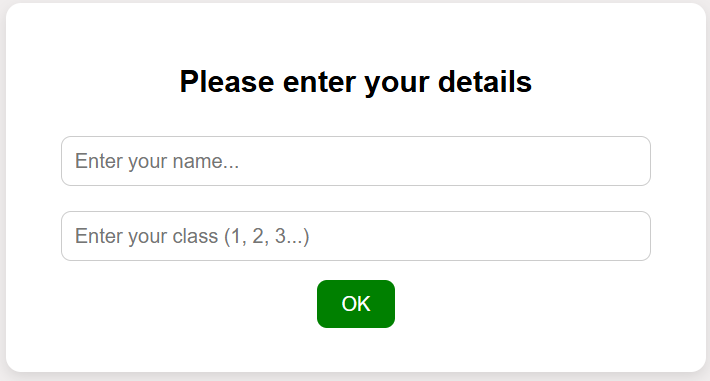
\includegraphics[width=\linewidth]{first.png}
    
    \label{fig:minipage1}
  \end{minipage}
  \hfill
  \begin{minipage}{0.45\textwidth}
    \centering
    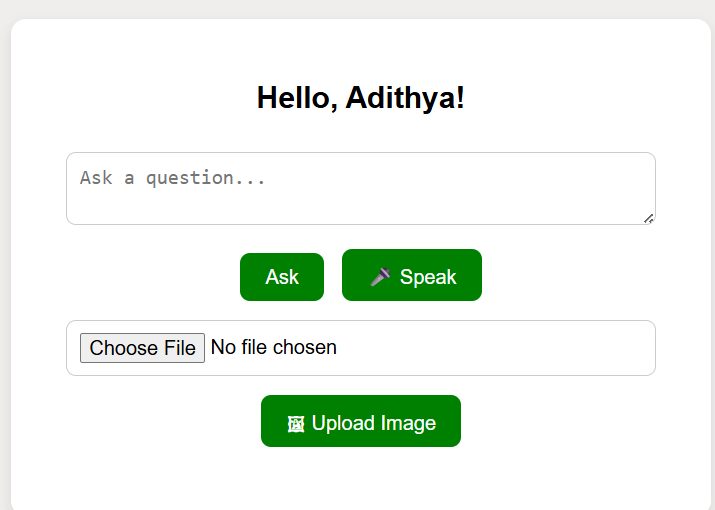
\includegraphics[width=\linewidth]{second.png}
    
    \label{fig:minipage2}
  \end{minipage}

\end{figure}

\begin{figure}[h]
  \centering
  \begin{minipage}{0.45\textwidth}
    \centering
    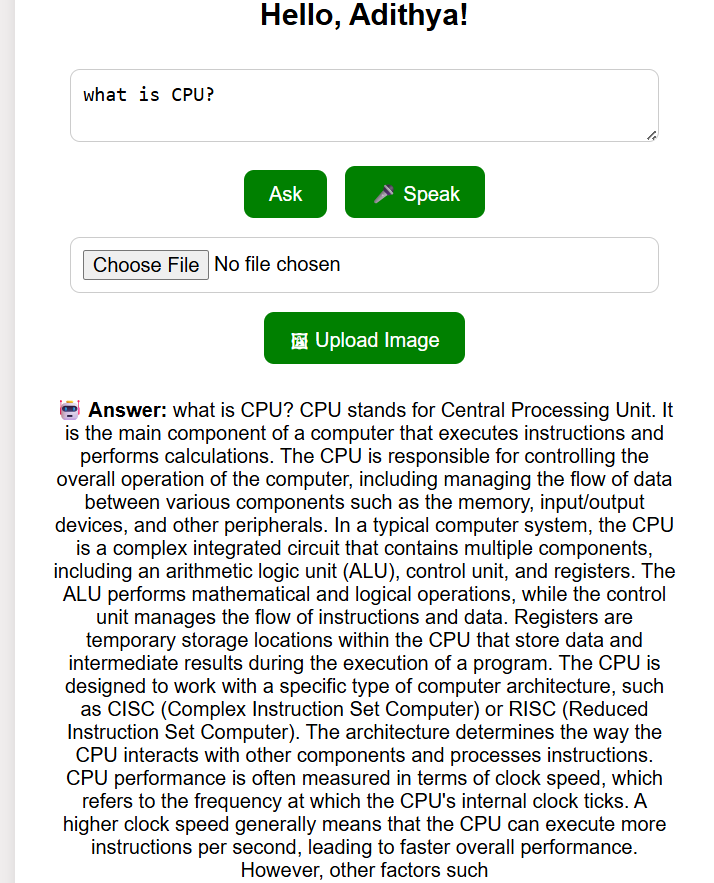
\includegraphics[width=\linewidth]{third.png}
    
    \label{fig:minipage1}
  \end{minipage}
  \hfill
  \begin{minipage}{0.45\textwidth}
    \centering
    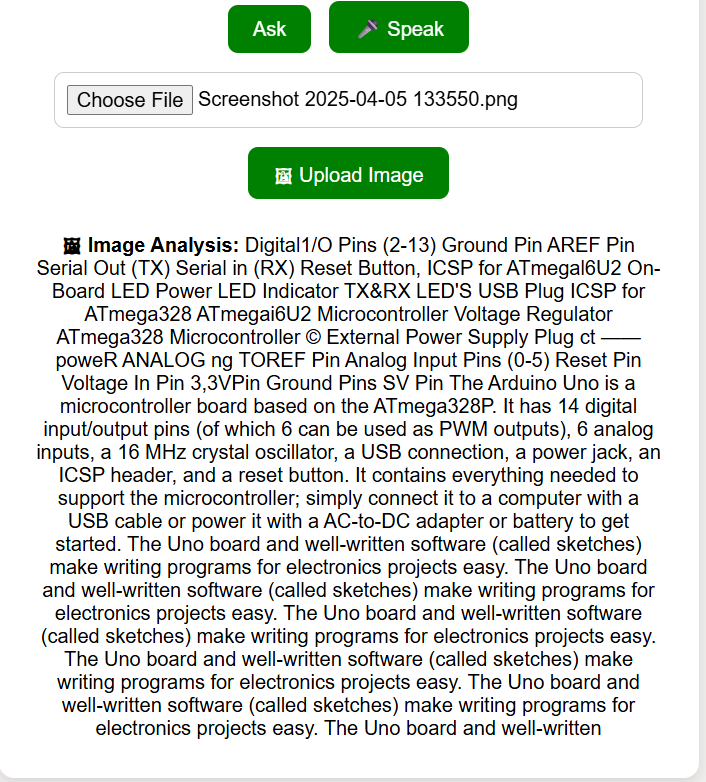
\includegraphics[width=\linewidth]{fourth.png}
    
    \label{fig:minipage2}
  \end{minipage}
\end{figure}
\section*{Acknowledgments}
I would first like to express my heartfelt gratitude to the Intel Unnati team for providing valuable resources, technical support, and an excellent platform to work with advanced AI frameworks. Their initiative enabled me to gain hands-on experience in developing intelligent systems, which played a significant role in the successful completion of this project.
I extend my sincere thanks to Mr. Siju Swamy, my project mentor, for his continuous guidance, encouragement, and insightful suggestions throughout the project. His expert advice and constant motivation were vital to every stage of this work.
I am also grateful to my guide, Mr. Anish Sir, for his consistent support, timely feedback, and valuable input, which helped refine and improve this project effectively.
I would like to thank Saintgits College of Engineering for providing a conducive academic environment, technical facilities, and all the resources necessary to complete this project successfully.
Finally, I sincerely thank my family and friends for their unwavering encouragement, moral support, and motivation throughout this journey.
\cite{brownlee2019}
\begin{thebibliography}{8}

\bibitem{brownlee2019}
Brownlee, J. (2019). \textit{Deep Learning for Natural Language Processing: Develop Deep Learning Models for Text Data in Python}. Machine Learning Mastery.

\bibitem{chollet2017}
Chollet, F. (2017). \textit{Deep Learning with Python}. Manning Publications.

\bibitem{grinberg2018}
Grinberg, M. (2018). \textit{Flask Web Development: Developing Web Applications with Python}. O'Reilly Media.

\bibitem{openvino}
OpenVINO\textsuperscript{TM} Toolkit Documentation. [Online]. Available: \url{https://docs.openvino.ai}

\bibitem{huggingface}
Hugging Face Transformers Documentation. [Online]. Available: \url{https://huggingface.co/docs/transformers}

\bibitem{pytesseract}
Pytesseract: Python-tesseract OCR Tool. [Online]. Available: \url{https://github.com/madmaze/pytesseract}

\bibitem{flaskdocs}
Flask Documentation. [Online]. Available: \url{https://flask.palletsprojects.com/}

\bibitem{webspeechapi}
Web Speech API — MDN Web Docs. [Online]. Available: \url{https://developer.mozilla.org/en-US/docs/Web/API/Web_Speech_API}

\end{thebibliography}
\appendix
\section{Main code sections for the solution}
\textbf{Model Initialization and Compilation}
 This part loads the language model and tokenizer from the INT8-optimized neural-chat model directory and compiles the model using OpenVINO for fast inference.


 
\begin{python}
tokenizer = AutoTokenizer.from_pretrained("neural-chat/INT8")
ov_model = OVModelForCausalLM.from_pretrained("neural-chat/INT8", device="CPU", compile=False)
ov_model.compile()
print("Model compiled and ready.")

\end{python}
\subsection{Flask App Configuration }
The Flask server is set up to serve static files (frontend), handle CORS, and define a directory to store uploaded images. 
\begin{python}
app = Flask(__name__, static_folder="frontend", static_url_path="/")
CORS(app)
UPLOAD_FOLDER = "uploads"
os.makedirs(UPLOAD_FOLDER, exist_ok=True)
app.config["UPLOAD_FOLDER"] = UPLOAD_FOLDER

\end{python}
\subsection{Chat Route for Text Queries (Backend) }
Handles POST requests with a users text input, processes it with the tokenizer, generates a response from the model, and sends it back in JSON.

 
\begin{python}
@app.route("/chat", methods=["POST"])
def chat():
    question = request.get_json().get("question", "").strip()
    inputs = tokenizer(question, return_tensors="pt")
    outputs = ov_model.generate(**inputs, max_new_tokens=256)
    response = tokenizer.decode(outputs[0], skip_special_tokens=True)
    return jsonify({"answer": response.strip()})

\end{python}
\subsection{OCR \& Image Upload Handler  }
Accepts image uploads, extracts text using pytesseract, and generates AI responses from the extracted content. 
\begin{python}
@app.route("/upload-image", methods=["POST"])
def upload_image():
    image = request.files["image"]
    image_path = os.path.join(app.config["UPLOAD_FOLDER"], secure_filename(image.filename))
    image.save(image_path)
    extracted_text = pytesseract.image_to_string(Image.open(image_path), lang="eng").strip()
    inputs = tokenizer(extracted_text, return_tensors="pt")
    outputs = ov_model.generate(**inputs, max_new_tokens=256)
    response = tokenizer.decode(outputs[0], skip_special_tokens=True)
    return jsonify({"answer": response.strip(), "extracted_text": extracted_text})

\end{python}   




\subsection{Frontend Layout Design (HTML/CSS) }
The UI is divided into three stages: a splash screen, a form to collect user details, and the main Q\&A interaction page. Styled using CSS.

 
\begin{python}
<div id="introPage" class="container">WELCOME TO MENTORA</div>
<div id="page1" class="container" style="display: none;">
  <input type="text" id="nameInput" placeholder="Enter your name...">
</div>
<div id="page2" class="container" style="display: none;">
  <textarea id="questionInput" placeholder="Ask a question..."></textarea>
</div>

\end{python}
\textbf{Splash Screen and Page Navigation}  }
Controls the automatic transition from splash screen to user input form after a delay.

 
\begin{python}
window.onload = function () {
  setTimeout(() => {
    document.getElementById("introPage").style.display = "none";
    document.getElementById("page1").style.display = "block";
  }, 3000);
};

\end{python}
\subsection{Fetching AI Response for Typed Questions }
Captures user’s typed question and sends it to the backend’s /chat endpoint. The result is displayed below.

 
\begin{python}
async function getAIResponse() {
  const question = document.getElementById("questionInput").value.trim();
  const res = await fetch('/chat', {
    method: 'POST',
    headers: { 'Content-Type': 'application/json' },
    body: JSON.stringify({ question })
  });
  const data = await res.json();
  document.getElementById("responseBox").innerHTML = `�� Answer: ${data.answer}`;
}

\end{python}
\section{  Main code for model}
\subsection{Image Upload \& Answer Display  }
Submits the uploaded image to the backend for OCR and displays the resulting answer.

 
\begin{python}
function uploadImage() {
  const file = document.getElementById('imageInput').files[0];
  const formData = new FormData();
  formData.append('image', file);
  fetch('/upload-image', {
    method: 'POST',
    body: formData
  })
  .then(res => res.json())
  .then(data => {
    document.getElementById("responseBox").innerHTML = `�� Image Analysis: ${data.answer}`;
  });
}

\end{python}
\subsection{Voice Input Using Web Speech API  }
Enables users to speak their questions. Captures speech, converts it to text, and fills the input box.

 
\begin{python}
function startVoiceInput() {
  const recognition = new (window.SpeechRecognition || window.webkitSpeechRecognition)();
  recognition.lang = 'en-US';
  recognition.start();
  recognition.onresult = function (event) {
    const transcript = event.results[0][0].transcript;
    document.getElementById("questionInput").value = transcript;
  };
}

\end{python}
  

\subsection{Dynamic User Flow \& Personalization }
Handles storing the user name/class and moves them into the chat interface for a more personalized experience.

 
\begin{python}
function goToNextPage() {
  const name = document.getElementById("nameInput").value.trim();
  const classNumber = document.getElementById("classInput").value.trim();
  document.getElementById("studentName").textContent = name;
  document.getElementById("page1").style.display = "none";
  document.getElementById("page2").style.display = "block";
}

\end{python}
\end{document}
